%--------------------------------------------------
% Survival Guide
%--------------------------------------------------
\documentclass[letterpaper,11pt]{report}

%--------------------------------------------------
% Declaration section
%--------------------------------------------------
\usepackage{graphicx}
\usepackage{subfigure}
\usepackage[pdfauthor={GuyGuy}, pdftitle={Survival Guide}, pdfsubject={Software Manual}, pdflang={English}]{hyperref}
\usepackage{amsmath}
\usepackage{amssymb}
\usepackage{listings}
\usepackage{textcomp}
\usepackage{color}
\usepackage[usenames,dvipsnames]{xcolor}
\usepackage[margin=1in]{geometry}
\usepackage{ccaption}
\usepackage{times}
\usepackage{fancyhdr}
\usepackage{lastpage}
\usepackage{url}
\usepackage[hyphenbreaks]{breakurl}
%\usepackage{mnsymbol}
\usepackage{tikz}
\usepackage{enumitem}

\setlist{nolistsep}

\hypersetup{linktocpage=true,colorlinks=false,linkcolor=blue,citecolor=blue,pdfpagemode=UseNone,pdfstartview={XYZ 1000 1000 1}}

% Change the format of a figure caption
% For more options see the package documentation
\captionnamefont{\bfseries}
\captiontitlefont{\small}
\captiondelim{ --- }
\hangcaption
\renewcommand{\figurename}{Figure}

\renewcommand{\thesubfigure}{\thefigure.\arabic{subfigure}}
\makeatletter
\renewcommand{\p@subfigure}{}
\renewcommand{\@thesubfigure}{\thesubfigure:\hskip\subfiglabelskip}
\makeatother

\hypersetup{linktocpage=true,colorlinks=false,linkcolor=blue,citecolor=blue,pdfpagemode=UseNone,pdfstartview={XYZ 1000 1000 1}}

\definecolor{dkgreen}{rgb}{0,0.6,0}
\definecolor{gray}{rgb}{0.5,0.5,0.5}
\definecolor{mauve}{rgb}{0.58,0,0.82}
 
\lstset{ %
  basicstyle=\ttfamily \footnotesize,           % the size of the fonts that are used for the code
  numbers=left,                   % where to put the line-numbers
  numberstyle=\tiny\color{gray},  % the style that is used for the line-numbers
  stepnumber=1,                   % the step between two line-numbers. If it's 1, each line 
                                  % will be numbered
  numbersep=5pt,                  % how far the line-numbers are from the code
  backgroundcolor=\color{white},      % choose the background color. You must add \usepackage{color}
  showspaces=false,               % show spaces adding particular underscores
  showstringspaces=false,         % underline spaces within strings
  showtabs=false,                 % show tabs within strings adding particular underscores
  frame=single,                   % adds a frame around the code
  rulecolor=\color{black},        % if not set, the frame-color may be changed on line-breaks within not-black text (e.g. commens (green here))
  tabsize=2,                      % sets default tabsize to 2 spaces
  captionpos=b,                   % sets the caption-position to bottom
  breaklines=true,                % sets automatic line breaking
  breakatwhitespace=false,        % sets if automatic breaks should only happen at whitespace
  title=\lstname,                   % show the filename of files included with \lstinputlisting;
                                  % also try caption instead of title
  keywordstyle=\color{blue},          % keyword style
  commentstyle=\color{dkgreen},       % comment style
  stringstyle=\color{mauve},         % string literal style
  escapeinside={\%*}{*)},            % if you want to add a comment within your code
  morekeywords={*,...}               % if you want to add more keywords to the set
}

%--------------------------------------------------
% Headings
%--------------------------------------------------
\fancypagestyle{plain}{
\fancyhead{} % clear all header fields
\fancyhead[LO,RE]{\normalsize \slshape Left 4 Dead Survival Guide}
\fancyhead[RO,LE]{\normalsize \slshape \leftmark}

\fancyfoot{} % clear all footer fields
\fancyfoot[LE,RO]{\normalsize \thepage\ of \pageref*{LastPage}} % insert page numbers
\renewcommand{\headrulewidth}{0.7pt}
\renewcommand{\footrulewidth}{0.7pt}
}

\renewcommand{\sectionmark}[1]{\markboth{\thesection.\ #1}}

\setcounter{tocdepth}{2}

%--------------------------------------------------
% Document Environment
%--------------------------------------------------
\begin{document}

\pagenumbering{roman}
\begin{titlepage}
\begin{flushright}
\footnotesize
Written by: \texttt{guyguy}
\today
\end{flushright}

\vspace*{\fill}
\begin{center}
\begin{tikzpicture}
	\draw (0, 0) node[align=center, inner sep=0] {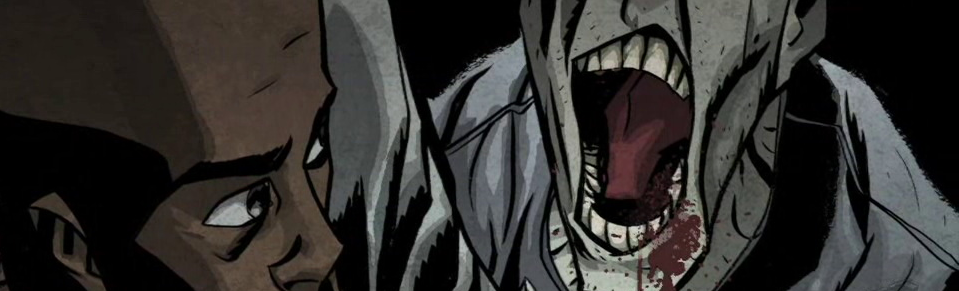
\includegraphics[width=\columnwidth]{cover}};
	\draw (0, 1) node[align=center] {\textsc{\huge \color{White} Left 4 Dead Survival Guide}};
\end{tikzpicture}
\end{center}
%\tableofcontents
\vspace*{\fill}
\end{titlepage}
\newpage
\pagenumbering{arabic}
\pagestyle{plain}

\tableofcontents
%\listoftables
%\listoffigures
%\newpage

\pagestyle{plain}
\chapter{Introduction}
This document explains the strategies used for Left 4 Dead and Left 4 Dead 2 survival mode. I wrote a lot of these strategies down for the group ``North American Survivors'' and because I enjoyed doing so, I wanted to record them in a more permanent spot. This document is a work-in-progress. It's time consuming to write down all the details of the strategies used and there are also multiple strategies in many of the maps. Some of the maps do not have many details in this document, but this will hopefully be changed in the future.

\section{Purpose}
When first starting off with the game, it might seem that survival mode has very little depth, does not last very long, and is tedious and repititious. On the contrary, survival mode offers intense, challenging, and fun games with a lot of replayability, however, there is a lot of teamwork and strategy required. New players have not been exposed to the teamwork and strategy when they first start off, and perhaps even encounter people trying to exploit or ``glitch'' their way to gold medals on survival mode. This document will serve as a guide to new players and veteran players alike who want to see a thorough explanation of the survival strategies that they can use in their games with the right team of players.

There are many people playing survival mode in Left 4 Dead and Left 4 Dead 2 from all over the world, and it is a good opportunity to make new online friends and collaborate with them towards a common goal. The Left 4 Dead series are known to be high quality cooperative games that stress teamwork, and the addition of goals and records makes the game refreshing and endlessly replayable for many survival enthusiasts.

\paragraph{Other Game Modes?}
This guide applies to survival mode only. A lot of the strategies rely on how the A.I. work on the map and where the A.I. spawn and although some of the strategies may carry over to versus, versus survival, or scavenge, a lot of them will be ineffective. This strategies will easily apply to campaign mode, however, campaign mode is much easier due to the fact that the tanks do not spawn with horde of common infected. Campaign mode simply does not require such detailed strategies.

\section{Left 4 Dead or Left 4 Dead 2?}
Each of the two games have a very distinct flavor in survival mode. Left 4 Dead is a short-range map where the focus is on positioning to block chokepoints and to use the ammo conservatively. Left 4 Dead 2 is more long-range and there is more mobility involved. Overall, Left 4 Dead 2 is the more difficult game, however, some maps in Left 4 Dead 2 are easier than maps in Left 4 Dead. Some players prefer one game over the other, but I personally enjoy both games. New players can begin in either game.

\section{Format of this Guide}
The guide contains one section for each of the maps in both Left 4 Dead and Left 4 Dead 2. First, the positions that each of the four players should use are listed. Then, a number of helpful comments about the strategy are provided as notes.

\section{Acknowledgements}
Thanks goes to \texttt{TheKevSham}, \texttt{Licksore}, and \texttt{sauce} who wrote some of these strategies.

\chapter{Left 4 Dead}
This section will detail the strategies for Left 4 Dead.

\section{Weapons}
All the strategies (with a special exception of the gas station strategy) use the autoshotgun. At first thought, this might seem a little close-minded, but simply put, the autoshotgun is a more powerful weapon of Left 4 Dead and it is by far the best weapon choice for survival mode.

While it is possible and even a little more fun for experienced players to try the m16, the highest times will always be achieved using the shotgun.

\section{Map Difficulty}
The maps in Left 4 Dead survival have various levels of difficulty due to the level design and the given supplies. Here is an approximate ranking of the survival maps from easiest to hardest:
\begin{enumerate}
\item Street
\item Farmhouse
\item Gas Station
\item Generator Room
\item Construction Site
\item Port
\item Terminal
\item Drains
\item Warehouse
\item Hospital
\item Bridge (CC)
\item Bridge (BH)
\item Church
\item Boathouse
\item Lighthouse
\item Rooftop
\item Traincar
\item Runway
\item Truck Depot
\item Crane
\end{enumerate}

This should serve as an approximate guide for new players on which maps to try out first. While it's definitely not mandatory to play the maps in this order, new players will find the most success in the easiest maps and may find the harder maps very difficult and not fun until they have some experience with the easier maps.

\section{General Strategy}

\subsection{Ammo Runs}
In Left 4 Dead, there are breaks inbetween the waves of tanks. This is the opportunity when the survivors are able to make a run to replentish their ammo at the ammo pile. The times are:
\begin{itemize}
\item 1:30
\item 2:30 (optional)
\item 4:00
\item 6:00
\item 9:00
\item 12:00
\item 14:30, 16:30, and every two minutes afterwards
\end{itemize}

\section{No Mercy}

\subsection{Gas Station}
\paragraph{Positions}
\begin{itemize}
\item 1 player sniping, guarding the ladder
\item 1 player sniping, guarding the lift
\item 2 players shotguns, controlling the common infected
\end{itemize}

\paragraph{Notes}
\begin{itemize}
\item Communication is important for this strategy, especially when tanks are coming from two sides or tanks are dropping from the roof.
\item Shotgunners use pistols and shotguns to control the majority of the common infected. The snipers do not pay attention to any common infected and focus on sniping the special infected and tanks.
\item We try to keep the gas station intact and avoid blowing it up. However, stray bullets have always seemed to occur!
\item We have tried two variations for the shotgunners: the first is to use the shotgun as much as possible to clear horde and go for ammo run frequently. The other is opposite; try to use pistols as much as possible to clear the horde (with a little more difficulty), and go for ammo runs infrequently. The latter strategy seems to work to best because you can choose the ammo runs when there is a lull in the action, rather than forcing frequent ammo runs.
\item Dodging rocks is key to achieving high times. The shotgunners should not be stationary, since this will leave them open to get hit by long-range rocks.
\end{itemize}

\paragraph{Additional note: ladderblocking}
This strategy involves one of the snipers guarding over the ladder where common, special infected, and tanks may climb. The player can either stand over the ladder (ladderblocking), or melee/shoot zombies as they reach the top of the ladder. Blocking specials and tanks is ineffective because there's a good chance they will push you off the ladder to injure you. In the past there has been some debate whether ladderblocking should be allowed on this map or not. Our group as well as other North American players have always been on the side to allow ladderblocking of common infected, whereas some other players have been against it.

In this game we did not use ladderblocking, but infact we may chose to employ it in the future. I would like to point out firstly that it makes absolutely no difference in terms of the difficulty and implementation of the strategy. Ladder blocking is a game mechanic that is in both Left 4 Dead 1 and 2. It is caused from the fact that common infected will be killed when survivors land ontop of them. I have not seen a valid arguement against ladderblocking.

\subsection{Generator Room}
\paragraph{Positions}
All players are lined up against the wall.

\subsection{Hospital}
This is a very cramped map with difficult ammo runs. All players are camping inside the room with the hospital beds.

\subsection{Rooftop}
We were aiming for 40 minutes and were pleased to get further. The server/director was not giving us any breaks, sending a lot of double tanks and more special infected than the current world record of an hour. For me it was a really fun round and put our teamwork to the test. I recall someone getting hit off the building at least once and luckily being incapped instead of dying. Video: \url{http://youtu.be/BUV7dOql54c}

\paragraph{Positions}
\begin{itemize}
\item 1 Player front left
\item 1 Player front right
\item 1 Player front middle
\item 1 Player back
\end{itemize}

\paragraph{Notes}
\begin{itemize}
\item This video shows good positioning for dealing with tanks coming from left, front, and right side. Watch the ammo count closely to get a feel of how many bullets need to be expended on the tank and how to reload in time to deal with double tanks: \url{http://www.youtube.com/watch?v=b95BuBzRij4}
\item Certain positioning against the wall can allow you to merely take damage and avoid getting punched off the building.
\item Wait for the horde to climb up before meleeing or clearing them out with a few shots. All the zombies climb, which is can be easily controlled. Save the shotgun shells for hunters and tanks.
\item If a hunter pounces while the tank is climbing, priority is to kill or deadstop the hunter and then finish off the tank.
\item For us, the back player helps with tanks on the right, since the left player might be occupied defending the left and front
\item Rooftop is a map that normally is relentless with the tank spawns. Similar to church, killing the tanks that appear during ammo runs is vital. The mounted gun can be used to distract the tanks if needed.
\end{itemize}

\section{Death Toll}

\subsection{Drains}
This map is very buggy in the sense that tanks get stuck regularly. It is a poorly designed map for survival and is not played very often at all.

\subsection{The Street}
\paragraph{Positions}
\begin{itemize}
\item 3 players watch the front in a staggered line (rightmost in front)
\item 1 player watching the back
\end{itemize}

Rightmost player used 3 medkits. Middle player used 1 kit. The remaining players used 2 kits. We didnt start healing until about 50 minutes (and by an hour only 1 kit had been used).

\paragraph{Notes}
\begin{itemize}
\item Avoiding damage from rocks is key to getting high times. All rocks should be dodged or shot. The rocks can be avoided by moving towards the surrounding walls. It's a little precarious for the middle player to dodge rocks, so the positioning should be such that the tank throws rocks at the rightmost or leftmost player as much as possible.
\item The back position is tedious, but it's very important for the back player to be able to clear out the back of zombies and avoid smokers as much as possible. This is so that the front players can work without interference.
\item Smokers are dangerous if they are overlooked. They can separate the group and can cause damage. Shooting the tongue will prevent the smokers from having any effect.
\item Pistols were used a little, but we went for ammo runs regularly.
\item At the end, we put the player with least health at the back.
\item We went for extra pipebombs at the far end of the map at the beginning of the round. One was thrown to prevent us from getting horded at the beginning.
\end{itemize}

Because of the open area, tank rocks are a major source of damage, similarto the terminal map. The player on the left will be targeted the most by tank rocks. An easy way of avoiding damage is to strafe left towards the wall. The tank will try to compensate and actually throw the rock at the wall. Shooting the rocks is an alternative to dodging them, but I prefer not to because the rocks are not visible at a distance when graphics settings are on low. Dodging rocks is also reliable at a closer range than shooting rocks.

A useful skill for this map is getting midair shots (also known as ``skeeting''). Going for midair hunter kills is infact a low-risk manoeuvre since one can follow up the shot with a melee swing. In this map, the hunters will start pouncing the survivors from a long distance and they are moving in straight lines. A lot of hunters will go after the player on the right so he should be well-practiced at this.

During rare times you can get double tanks rushing in. Don't panic, they're quite manageable. You can keep your distance so that the tanks will take time to throw rocks instead of rushing in. The back area should be carefully cleared of zombies while the tanks are rushing in so that there is enough room to maneuver.

\subsection{Boathouse}

\subsection{Church}
Here's a map we've been playing a lot recently and have been making improvements. The previous record was broken on other occasions; accident and Domino have gotten 35 minutes on this map. Most of the improvements that need to be made on this map are dealing with the double tanks and late tanks.

\paragraph{Positions}
\begin{itemize}
\item 1 Player at the hole
\item 1 Player guarding the small room
\item 1 Player guarding the back
\item 1 Player on the piano standing on the piano keys
\end{itemize}

\paragraph{Notes}
\begin{itemize}
\item Similar to crash course bridge, the situation can turn ugly fast when a lot of zombies get through. It is important to block up the entrances at all possible times, such as when you are picking up an incapped player.
\item There is a wooden railing at the back position. I like to have the back player stay behind the wooden railing to prevent any chance of being smoked out the window. It also allows you to lead the in a tanks slightly different path.
\item Smokers are problematic if players get smoked out of the building. To prevent this, the player at the hole and at the small room can hide behind walls, peeking out occasionaly to shoot zombies. The piano player must also be careful not to get pulled out of the building.
\item After 30 minutes, the spawning rates are noticeably slower.
\item We went for ammo in groups of two, which seemed to help.
\item Double tanks seem difficult to deal with because as the players position themselves to shoot the tanks, horde slip through the unguarded entrances.
\item Tanks can be delayed once they climb the roof of the church. It seemed oftentimes that the tank would land at the back after climbing the roof. Late tanks are disruptive to the ammo runs.
\end{itemize}

The two front entrances receive a lot of incoming horde. This might actually seem overwhelming, but infact the zombie horde can be controlled by the one player per entrance. For the hole player, all zombies are forced to climb the sandbags because entering and for the small room player, the zombies are forced through a small doorway. The role of the piano player is to backup the others when they are smoked or pounced. He does not have to help kill common zombies at the three guarded entrances because it is of little use. The piano player should ensure that no common infected are seeping through the unguarded windows (rare event) and also should have 10 shots loaded to blast the tank with.

\section{Dead Air}

\subsection{Construction Site}
\paragraph{Positions}
\begin{itemize}
\item 1 player on the left side focusing left.
\item 1 player on the right of the left player focusing both sides.
\item 1 player on the left of the right player focusing both sides, also on top of a piece of wood to be slightly elevated.
\item 1 player on the right side focusing right.
\end{itemize}

\paragraph{Notes}
\begin{itemize}
\item Less ammo runs = less damage, it worked out nicely.
\item You and your team will be smoked constantly so be aware of your teammates and call for help.
\item The elevated player is more likely to spot a tank before others make sure that player is confirming which direction the tank is coming from.
\item It’s best to go for ammo after a tank/double tank is killed but make sure one isn’t on his way before you go. 
\item Shoot the boomer before falling for ammo and cover each other getting and returning from ammo.
\item Dodging rocks can be very difficult but the left guy must try.
\item Gas cans may be collected and stored where they won’t get shot but it’s really not necessary. 
\item There are only 3 pipe bombs on this map so use them very wisely when shooting for a high time.
\item Extra supplies are above you so go up when safe enough to do so.
\item If the tank climbs up one side it’s not always that he will come down same side he did last time. 
\item Save pills for quick health needed during an ammo run.
\item If the tank gets stuck 1-2 players should pistol him down otherwise you will get an embarrassing tank count.
\item Communication is very important call tanks, help, smoked, pills, etc.
\item Practicing with the same team over and over again will give you the best results.
\end{itemize}

\subsection{Crane}
We were really determined to get 30 minutes on this map and it took a lot of tries. We were getting consistent 20 minute times but kept getting destroyed before being able to heal or get ammo. Much of the problems had to do with the ammo runs; I figured out a rough plan for the ammo runs which I think helped. The map definitely feels as though it gets easier after 20 minutes, possibly due to special infected getting stuck. Conserving the medkits better within the first 20 minutes will help us approach the world record of 40 minutes. Also, I think the front and back corner have very specialized positions as will be explained.

\paragraph{Positions}
\begin{itemize}
\item 1 Player covering front (against the chimney)
\item 1 Player covering back in the corner (tongue cutter)
\item 2 other players complete the square-like formation
\end{itemize}

\paragraph{Notes}
\begin{itemize}
\item The front player is mostly focused on the front and rarely helps the back.
\item The back player is responsible for shooting the smoker tongues to free players as he will not be smoked often.
\item The front player must handle most of the zombies at the front. He must also deadstop the hunters that pounce him from the fence because this will stumble the rest of the players.
\item Of key importance is to free players from smoker tongues as fast as humanly possible. This is to prevent players from falling off the roof and also important so that players get enough shots into the tanks.
\item I prefer shooting the smoker tongues to break them as opposed to meleeing them. This is because shooting seems easier to time and you dont have to move out of position to cut the smoker tongue. The expense of 1 or 2 shotgun shells is negligible.
\item It is very easy to run out of ammo at the time between 9 and 12 minutes. At 9 minutes we go for ammo and stay at the ammo pile for about 20 seconds using ranged weapons.
\item We skipped approximately two ammo runs after 20 minutes. One was the ammo run at 28:30, which possibly got us killed but guaranteed us to get a time of 30 minutes. Although the spot seems to be too hectic to use pistols, the pace slows down after 20 minutes, allowing us to save on ammo.
\item There is a lot of fire available to be used in the map, and it sometimes is useful for the ammo runs.
\end{itemize}
\begin{itemize}
\item Second guy should be first back down and sit in front half of the cage and cover the run back of everyone else, using the vent to juke smokers tongues.
\item Also with tanks from the crane, don't all back into the corner, try to fan out enough so that you don't get multi-hits from the tank as this can also be game ending. If the guy on the back fence runs to wall directly under the crane he can crouch next to it to avoid being hit off, but this move is risky.
\item I agree with just shooting smokers tongues, often your first attempt to free someone with melee will not register so you can easily fatigue yourself doing this.
\item Also the guy in the corner can meatshot hunters to make them (cull)jump away from the cage before they enter.
 \item I find it easier to hide a little bit behind the vent as the front guy so the smokers go for the guy covering the window, and the guy covering the window should never need to help with any tanks from the front. You only ever need 4 people shooting a tank if it comes off the crane or you have doubles rock up at the same time.
 \item You can conserve ammo by having the guy on the back fence and in the corner of the cage use pistols whilst the other two use shotguns and switching positions. But this requires the ability to be able to play multiple positions.
 \item If using ranged weapons, it really should only be the first guy up to the ammo and he should use them till the last guy gets ammo and immediately follow him, and first up once up should always immediately check opposite building for smokers. as they can pull you off from there which can be a game ender.
\end{itemize}

\paragraph{Tank Strategy}
\begin{itemize}
\item If the tank is coming from the front, we hold our position and do not rush it. The tank will throw rocks that can be avoided by hiding behind the chimney or the crane ladder. When the tank approaches, the front player should have 10 shells ready to unload into the tank. The front player should be doing the most damage to the front tank because he has the best view of it.
\item If the tank is coming from the back, he will climb the fence. This is usually easy for 3 players to kill the tank as he is climbing.
\item If the tank is dropping from the crane, we press up against the fence to increase distance from the tank. We take some potshots as it is ontop of the crane and unload the brunt of the damage as it lands on the ground.
\item The tank may appear during the ammo run. If that happens, we try to kill the tank as we are getting ammo. The ammo pile is actually defensible for a short period of time, so it is not unreasonable to kill the tank during ammo run.
\item Ideally the tanks should be dead before reaching any player. Maximum one punch should be allowed to go through.
\end{itemize}

\paragraph{Ammo Run Strategy}
\begin{itemize}
\item If fire is to be used, it should be thrown into the small room where specials spawn in order to kill them faster. Flaming hunters must be dealt swiftly.
\item If there is extra time, a player at the ammo pile can pick up a ranged weapon and shoot the specials.
\item Players can reach the ammo within two jumps. This should be practiced.
\end{itemize}

\subsection{Terminal}
After trying both out, we think that we've discovered the most effective positioning for us. The general style of play we like tends to favor dodging rocks more than shooting them and also favors delegating the task of horde control to a single or small number of players.

During this run our team got wiped out with reasonably high health and one medkit remaining. This leads us to believe the world record is possible in the future here.

\paragraph{Positions}
\begin{itemize}
\item 3 players in a staggered line starting from the van
\item 1 player on the luggage conveyor watching the right side
\end{itemize}

We ended up having to use 2 medkits by 30 minutes.

\paragraph{Notes}
\begin{itemize}
\item It's well known that the map is very buggy and that the difficulty level varies depending on how much the tanks are getting stuck. We tried to molotov the stuck tanks and snipe some of the stuck specials when it was convenient.
\item By playing more forward away from the back fence, we found that the tanks dropping in from behind occur rarely.
\item The first 20-30 minutes are the most difficult because the specials and horde come constantly. In order to reduce damage done the molotovs and pipebombs are very useful. You can molotov areas where common zombies are rushing in and hopefully avoid creating many flaming tanks and hunters.
\item Tanks from the front should be handled by the 3 front players while the right player deals with horde from the right.
\item Tanks from the right should be lead by the rightmost player to the others. Meanwhile, the leftmost player clears out common.
\item Dodging rocks is important here but can be difficult when there is horde in the way.
\end{itemize}

Double tanks can be tricky to deal with. If it is a tank coming from the right, it might be useful to lead in to the back counter so the tank climbs. However, an unsuccessful attempt at this caused us to wipe out!

\subsection{Runway}
In this map, the ammo runs can be quite difficult. The players have to run out where they are exposed to many specials and tanks may appear during the ammo runs.
\subsubsection{Plane Wing}
\paragraph{Positions}
All four players lined up under the plane wing

\subsubsection{Far Corner}
This is an alternate strategy for runway. The ammo runs are slightly longer and the horde is more difficult to control. However, there is more room to move around and the specials and tanks will not drop on you.
\paragraph{Positions}

\section{Blood Harvest}
\subsection{The Warehouse}
Warehouse has been avoided for a while since it has the most difficult ammo runs in the game. NAS has seen and studied other strategies, but we can all agree on one way of playing this map for now. We went through the doors and up the stairs to the far corner of the map. The general style of play we like tends to favor dodging rocks and tongues as well as delegating the task of horde control to a single player while the other 3 players focus the tank.Despite how difficult the ammo runs are the rest is fairly easy. 

\paragraph{Positions}
\begin{itemize}
\item 1 player faces the upstairs hall near the shelving/pillar.
\item 1 player faces the upstairs hall near the guard rail on the right.
\item 1 player faces both up and downstairs sitting in the furthest corner.
\item 1 player faces the downstairs at the top of the stair way.
\end{itemize}

\paragraph{Notes}
\begin{itemize}
\item We use pistols primary until a tank gets close enough to taste our shotguns.
\item Tanks from the front should be handled by 3 players while the right player deals with horde from the stairs.
\item Tanks from the right should be handled by 3 players while the left player deals with horde and avoids specials.
\item Our first ammo run is at 9mins and we stay near the ammo in a corner until 12mins for an easy trip with nearly no damage taken. Use shotguns from 9mins until you return upstairs after 12mins.
\item Once upstairs pistols are spammed and players do their best to avoid rocks and smoker pulls.
\item Checking on allies ammo helps the team prepare when an ammo run is needed. We like to have at least 40 shotgun shells before we run for ammo. 
\item If one is using too much ammo have that player switch positions with the player with the most ammo to maximize efficiency. 
\item These ammo runs require great speed and cover; so, you may have to kill 1 or 2 tanks just to get there let alone getting back. Stay together and communicate. Pipe bombs make all the difference, but try not to throw too many.
\item Make sure you pick up any supplies on the way for ammo. Forgetting could make or break a new time.
\item It's well known that the map is somewhat buggy and that the difficulty level varies depending on how many tanks you get. We shoot to kill all the stuck specials. 
\item If the tank takes too long to get to you it might lead to a frightening double tank. (Which we had about 3.)
\item Dodging rocks/tongues upstairs is key to saving your health in the long run but can be difficult when horde overwhelms, request help if needed.
\item Its very important to save an ally immediately when shooting for high times, no health wasted.
\item pills are best saved for emergency use on ammo runs, as it's very easy for all but the guy covering the stairs to avoid taking any damage in the holdout spot.
\item If you go for the set at the far opposite corner past the ammo throw an extra pipe and pick a new one up next to them. 
\item The best route to grab the set on the cabling wheel is to go around the back of the train car after grabbing ammo and looping around it. 
\item Throwing a pipe before you run into the starting room on the way to get ammo a few seconds before you run in will clear horde and allow you to get through that room without trouble.
\item Although you want to conserve ammo as much as possible, don't be afraid to use your shotgun on the run back (at least till you've got upstairs).
\item To conserve ammo with tanks pistol them till they get close/you need to reload your pistols (you can stretch ammo runs to once every 20 minutes even with a tank per min using this method).
\end{itemize}

\subsection{Bridge}
\paragraph{Positions}
\begin{itemize}
\item One on the couch covering back
\item One on the boxes covering back
\item One against the wall covering front
\item One ontop the table covering front
\end{itemize}

\paragraph{Notes}
\begin{itemize}
\item Although players are assigned areas to cover, all players must shoot the tank!!
\item Once the tank climbs, he will land on a random side. Therefore, voice communication has limited usefullness
\item The player on the box can dodge smoker tongues with slight movement
\item The player on the box should stay near the back once the smokers stop coming. This will make the tank climb the boxes
\item The player on the couch should stay at the top the couch
\item The two players near the ammo pile can spam the shotgun by picking up new weapons quickly
\item We are mostly certain that the pills in the medicine cabinet will not turn into medkits
\item Spawn rates are quite random on this map, but we had a good kill count
\item Since one inevitably takes damage on this map, it is good to heal as late as possible. We had about 2 people go black-and-white before healing
\item Using the explosives and gascans is ill-advised!!
\end{itemize}
Table position works differently than expected. The tank will very rarely climb the table but usually targets the person on the ground. More testing needed!

\subsection{Farmhouse}
\paragraph{Positions}
\begin{itemize}
\item 1 player covering back
\item 2 players covering hole
\item 1 player in the middle
\end{itemize}


\section{Crash Course}

\subsection{Truck Depot}
Another map that took many tries to get 30 minutes. This map is probably the second hardest in left 4 dead due to its randomness in zombie spawns. At times it can feel relatively easy and other times double tanks will end the game abruptly. We used the basically the same strategy as the Australians did so see Azimuth's video (\url{http://www.youtube.com/watch?v=B3fEeqK99HA}) or ask us for more details. This also leaves me with 30 minutes on all maps :)

\paragraph{Positions}
\begin{itemize}
\item 1 Player front sandbag
\item 1 Player front right sandbag
\item 1 Player front left sandbag
\item 1 Player back
\end{itemize}

\paragraph{Notes}
\begin{itemize}
\item Smokers pull players off the buses and are very disruptive.
\item This strategy is completely reliant on the smokers getting stuck after 12 minutes. Smokers naturally get stuck in unreachable areas when you hold at the sandbags. This might sound like a lame tactic, but it is sort of a quirk of truck depot. I'm certain that every high time achieved on truck depot had most of the smoker kills before 12 minutes and the smokers getting completely stuck sometime afterwards. If the smokers are still spawning after 12 minutes, you will struggle to reach 20 minute times.
\item Crouching behind the sandbags is generally a good idea to avoid getting pounced by hunters. However, it might cause you to fail to notice a tank climbing up
\item The back player must cover the entire back area. He can see both the left and right sides at the same time if he has a widescreen display.
\item Late in the game, tanks might come during the normal ammo run times (14:30 and every two minutes thereafter).
\item We tried to do a similar ammo run strategy that we used in crane, where we go for ammo in two passes. This seemed to help at times but other times it made the ammo runs slower than normal.
\item We used pistols to conserve ammo and skip the ammo runs at 24:30, 26:30, 28:30
\end{itemize}

\subsection{Bridge}
\paragraph{Positions}
\begin{itemize}
\item 2 players covering the hole (front)
\item 1 player covering the main entrance (back)
\item 1 player as support (covering hole in the wall)
\end{itemize}

\section{The Sacrifice}

\subsection{Traincar}
\paragraph{Positions}
\begin{itemize}
\item One person at the back as 'hunter fodder'
\item One person at the back corner covering back and hunter fodder, and any of the front players who may get pounced
\item One person front left side
\item One person front right side (a little further ahead of the left player)
\end{itemize}

\paragraph{Notes}
\begin{itemize}
\item Three players are shooting the tank at the front or back. The remaining player is covering the other side under normal circumstances.
\item Ammo runs after 12 minutes are sometimes inconsistent. Tanks may appear during ammo runs.
\item When going for ammo runs, it is sometimes best to use the fence to guide you to the ammo, while other times it is better to just run straight to the ammo pile. Be careful not to stay too close so as not to stumble each other if someone gets pounced.
\item It is difficult but not impossible to pick up incapacitated players in this spot.
\item Players at the back must be careful to dodge the tank rocks. This is difficult.
\item Players must be freed from smoker pulls as soon as possible. The cover player is better off shooting the tongues rather than meleeing to free the smoked player.
\item It's difficult to avoid scratches in the hunter fodder position. The best you can do is back up after you dead stop, or it may even be better to let yourself get pounced as long as the corner/cover player saves you fast enough for you to not take too much damage, if any.
\item Many times it is difficult to tell whether the tank is going to the front or back. The communication should be made last minute so not to confuse teammates.
\item Gascans and explosives are unnecessary.
\item The front players must back up from the tank to avoid getting hit. The front-right player leads the tank, so the front-left player backs up first. The timing of when to back up on this map is extremely finicky. Run back too early and the tank will climb the boat; run back too late and you will get hit. guyguy tried to measure the position of the tank by the shadow the tree in the corner makes upon the ground. By his judgment, the front-left player should back up just before the tank reaches the shadow. Just after the tank comes within the shadow, the front-right player should back up. It takes some practice to get used to.
\item If there is a double tank, however, you would want to manipulate one of the tanks to climb the boat while you deal with the other. 
\item Also interesting note, if you turn your settings down, the tall grass around the tree in the front isn't there, so you'll have an easier time seeing hunters that go in that spot.
\end{itemize}

\subsection{Port}
\paragraph{Positions}
\begin{itemize}
\item 1 person at the left door
\item 1 person on the railing at the top of the stairs guarding stairs/middle
\item 1 person on the right against the shelves watching the right side
\item 1 person on the left of the right-side player, against the railing, but watching the stairs.
\end{itemize}

By 33 minutes, no one had healed or hit 50hp even, so the first half hour was really smooth. By 50 minutes, someone had finally hit red health and everyone else was 50hp or below. We didn't run for med kits until about 64 minutes, not a very clean run but we made it back. We had some really great saves during this run, I had gotten smoked down to the street and was close to dying but was revived, a tank came while we were all still out there, and if I remember right, guyguy was 1hp during this time, and Azimuth had just gotten incapacitated. We made it back up to our holdout. Guyguy was black and white (at about 80 minutes?) so he stayed back towards me to be safe. At 83 mins, Azi was at 1hp. They both survived being that low on health until the end of the game. Not long later, Azi was black and white as well, Lone was a "damage sponge" on the right and I stayed at the left covering while guy and Azi stayed back to be safe. They also made several risky ammo runs while at 1hp. 

\paragraph{Notes}
\begin{itemize}
\item Guyguy suggested that we throw the gascans on the street outside of the left door because that's where the specials pile up, so we started doing that and it seemed to work nicely instead of throwing the gascan down the staircase (where sometimes it would land too closely and our positions would be on fire :P). 
\item The right-side player who plays against the railing keeps the tanks from dropping on the railing.
\end{itemize}

\section{Last Stand}
\subsection{Lighthouse}
\paragraph{Positions}
At the top of the lighthouse near the pipebimbs, not mollies. Everyone needs to stay crouched with their backs against the wall of the lighthouse tower. If you stand up or near the ledge you will either get smoked off or hunters will have an angle to pounce/stumble the team. It’s important to communicate since the tank needs to be killed instantly, he will surprise the team from 3 potential climbing locations (left, ladder, and right). Sometimes he will climb from the far left, or the far right, so be prepared to react quickly. Tanks climbing the ladder seem to come up faster.
\begin{itemize}
\item 1 Player sitting on the stack of pipe bombs (any further to the right leaves them vulnerable to smokers on the roof) covering the front and right.
\item 1 Player to the left of that person covering the front, right, and left side (this player is also the one who shoves smokers off to control the smoke).
\item 1 Player to the left of the previous position covering the front, right, and left side.
\item 1 Player to the left of the previous position covering the front and left side.
\end{itemize}

In the room with the fireplace, it’s important to communicate since the tank needs to be killed instantly, he will surprise the team from any direction. Tanks rarely come from the window, they're usually in the front or back, or sometimes the side room.
\begin{itemize}
\item 1 Player covering the front door facing the gun spawns.
\item 1 Player covering the window facing the gun spawns.
\item 1 Player covering the side door and back window.
\item 1 Player covering the wall that breaks down in the back.
\end{itemize}

\paragraph{Notes}
\begin{itemize}
\item Too many smokers climbing the ladder and dying at once will blind you with a thick smoke screen.
\item If a tank doesn’t die fast enough on the tower he will knock a survivor off the building, killing him, and ruining the rest of the game.
\end{itemize}

\paragraph{Ammo Run Strategy}
\begin{itemize}
\item Our first ammo run was at 9mins, then 12 and returning to the top of the lighthouse near the pipebombs.
\item We conserved our ammo until we had about 30 shells left. Once clear of a tank we pipe out get ammo then made our way back up to the lighthouse. Repeating until the 26:30 ammo time.
\item Deciding to keep it safe for our goal of 30mins we retreated and held the room with the fire place. Only getting ammo when it was clear.
\item After picking up the last medkit we looked for an opportunity to head back to the top to stretch it to 40mins. Around 30mins we piped and went to the top.
\item guyguy forgot to get ammo on his way up and died going back to retrieve it. Dying to a bullshit glitch pounce which could have been avoided if ammo wasn’t forgotten earlier.
\item Nearing our last shells we held until 40mins before risking another ammo run.
\end{itemize}
 
\chapter{Left 4 Dead 2}

\section{Map Difficulty}

\begin{enumerate}
\item Bridge
\item Mall Atrium
\item Generator Room
\item Gator Village
\item Bus Depot
\item Stadium Gate
\item Sugar Mill
\item Underground
\item Concert
\item Riverbank
\item Motel
\item Plantation
\item Traincar
\item Port (S)
\item Port (P)
\item Rooftop (No Run)
\item Burger Tank
\end{enumerate}

\section{Dead Center}

\subsection{Mall Atrium}
Mall Atrium is a unique map because of its design. It includes three floors that the players can move around in and therefore gives players and most mobility and flexibility in terms of effective strategies. There are two types of strategies in this map: running and holding. The running strategy involves running from the tanks in a circuit and the hold strategies are like the other traditional strategies where the players try to kill all of the tanks. The easiest strategy to begin with is the running strategy.

\subsubsection{Bridge Hold (with stairs)}
This strategy involves holding the bridge but having one person on the stairway. The change in positioning radically changes the AI pathfinding and causes tanks to run up the stairs instead of climbing the columns as they usually do. This video shows roughly the strategy used however, it was more of an improvised/testing run so infact the strategy is more organized at this point: \url{http://youtu.be/mSrCbEguBIM}.

\paragraph{Positions}
\begin{itemize}
\item 1 Player cover the top of the stairs
\item 1 Player on the stairs
\item 1 Player cover the bridge
\item 1 Player general/sniping
\end{itemize}

\paragraph{Notes}
\begin{itemize}
\item This positioning greatly frees up the space and freedom of movement on the top floor. However, the three top floor players must deal with the tanks without help from the fourth.
\item The player on the stairs has the most difficult position. He must fend off a lot of common zombies and avoiding getting hurt by specials and tanks going up the stairs
\item The player on the stairs must be carefully protected. The player guarding top should prevent zombies dropping at the top of the stairs onto him. Also do not bait tanks onto the stairs as this can be disasterous!
\item Depending on your positioning on the stairs, tanks will attack different. Move closer to the bottom and tanks will chase you up the stairs. Move close to the top and tanks will chase you up columns. Therefore, the stairs player has some control over the ebb and flow of tanks.
\item Gascans should be saved for the stairs player. The stairs player can kill a lot of zombies by flaming the stairs and baiting them to run through the fire.
\item Jockeys are difficult to deal with on the stairs and can cause you to take fall damage. The top floor players should lookout for the specials.
\item Players on the bridge need to watch for chargers that charge across the bridge.
\end{itemize}

\subsubsection{Saferoom Hold}
This is more of a hybrid strategy because it involves both running and killing the tanks. Many of us mallrats refer to the 3F enclosed area as the saferoom. Some of us malls rats have been working on and tweaking a strategy, which involves holding your teams position inside the saferoom, killing tanks, and going for ammo when neccessary.

This strategy (or variation) is a combined effort of Mallrats and 24 carat survival
(\url{http://steamcommunity.com/groups/24CtS}).

\paragraph{Setup}

\subparagraph{Supplies}

Bring all supplies including guns to the saferoom. (not absolutely necessary, but makes it easier). Separate to your liking all the supplies such that they are easily accessible while playing under pressure.

\subparagraph{Gascans}

Place gascans between the crevasse. (Note: gascans are not necessary or this strategy to work; however, the more the supplies the easier it is).

\paragraph{Positions}
\begin{itemize}
\item 2 Snipers in front of the entry way, a little behind the wood walls such that tank rocks, and chargers will not stumble you.
\item 1 Shotgun that focuses 90\% of his/her attention on the back wall.

\item 1 Swivel position that switches between shotgun and sniper depending on where the tank comes from.
\end{itemize}

\paragraph{Description}

\begin{itemize}
\item Front Entry way (front)
\item Back wall (back)
\item Drop hole (hole)
\end{itemize}

2 Snipers ( or 3 if the swivel is required to help the front), take out special infected and common infected in the hallway. The back shogun must make sure that no common or SI (special infected) get through to bother the 2 or 3 front snipers, especially chargers and spitters. If these SI get in the way it can be game over when the tank attacks.

\subparagraph{Front Tanks}
If the tank comes from the front, 2 Front snipers and 1 Swivel focus fire it. A tank takes approximately 45 sniper rounds to kill, which means 15 rounds per sniper (or 1/2 a clip). If the tank is still alive when entering the saferoom and if the back is clear, the back shotgun can blast a couple shells in to finish the tank off.

\subparagraph{Back Tanks}
If the tank comes from the back, the back shotgun IMMEDIATELY has to call the tank in order to alert the swivel if he/she is facing the front. You will know 80\% of the time the tank is coming from the back if the ground starts rumbling. While the tank is climbing up the back shotgun and swivel blast the tank with 10 shells each through the wall. The swivel then moves quickly out of the way such that the tank will lock onto the back shogun. The back shogun proceeds to move backwards towards the hole but onto the ledge, without dropping down. Once the shogun has reached the corner, the tank cannot attack him/her and must then move around the hole (refer to hole dance). While this is happening 1 sniper (left sniper) is always facing the front to deal with SI or common.

\subparagraph{Hole dance}
This requires the left front sniper to lead the tank towards the hole. towards the back. You can prevent yourself from dropping down the hole by hugging the left wall and you backtrack. Once the tank reaches the front side of the hole and the player is on the other end the tank will attempt to go around and hit you on the other side. At that point you will want to move back towards the front on the ledge and repeat until the tank is dead.

\subparagraph{Ammo}
Ammo runs are possible at the 3F bridge ammo before 12 mins.
After 12 mins, call out when ammo is running low and on the next tank perform a conventional circuit.

\paragraph{Acknowledgements}
Perhaps many people have come up with variations on this strategy; however, I would like to give credit to those who helped develop this particular variation. Unfortunately I am uncertain of absolutely everyone involved, but anyone knows anything please let me know and I will add to the list.

\begin{itemize}
\item Piling guns in saferoom: murphy
\item 1 swivel position: reminiscence
\item The hole dance: guyguy
\item Tweaks/Testing: phoenix\_advance, guyguy, kev, lone wolf macgruber
\item Stress Testing: arkron, clutch, benanigans, jester, lemonman, flux, trash4cash, logankenesis
\item Circuit: Kris and the members of randomgroup21 (\url{http://steamcommunity.com/groups/randomgroup21})
\end{itemize}

Video Example: \url{http://www.youtube.com/watch?v=2fWy_tB2qug}

\section{Dark Carnival}

\subsection{Motel}
No information written yet.

\subsection{Stadium Gate}
\paragraph{Positions}
When holding the roof top of the barn near the AK47 face the other rooftops as front so we have:
\begin{itemize}
\item 1 Player at the right of the rooftop.
\item 1 Player at the left of the rooftop.
\item 2 Players in between on the rooftop.
\end{itemize}
Soon tanks overrun us resulting in a fall back to the AK47 spawn so we have:
\begin{itemize}
\item All 4 Players near close enough to the gun spawn to avoid reloading.
\end{itemize}

\paragraph{Tank Strategy}
\begin{itemize}
\item Gun down the common and tanks almost the same time.
\item Pick up a new AK47 when near the gun spawn.
\item Avoid rocks by shooting them or dodging them.
\item You can get around the same amount of si kills without holding the roof, just by killing infected during breaks. When you hold the roof they tend to get stuck elsewhere. Also a well placed molotov can kill the si that are stuck, but you'll probably need to practice the throw a bit to get use to the angle.
\end{itemize}
We have a lot of room for improvement and ideas on the way to get more SI kills safely. Next time we need to deal with rocks better and conserve medkits longer. Until next time, I suppose we can shoot for an hour or while we are at it the world record.

\subsection{Concert}
This map may have had the most changes strategy wise due to not only the dispute over ladder blocking but the map changing all together. Since the update concert provided a better versus map, survival has had to adapt to new spawn points and old strategies crumbling. Although common infected are easy to kill and you'd rather focus on something like a special infected or tank(s) they serve an important role in the game. The combination of an endless horde, special infected, and tanks balance the games difficulty so removing one of these three would make a simple game. When all four play on the sniper tower it’s impossible for any common to play their role by blocking their climb. Not to mention the blocking of anything else climbing up. The description below is how we played concert to achieve the world record without blocking anything.

Description: (Moved Supplies)
One player was on the sniper spawn scaffolding and did not block any ladders. The three other players played near the 2 medkits at the top of the bleachers. We played this way for the majority of the round but the first 9 mins we defended the stage in hopes of a better special infected count. Common infected may be funneled in by the guard rails near those 2 medkits so one player is free of horde to focus on the tanks/ SI while the other 2 focus on not letting common in. 

\paragraph{Positions}
(Front is facing the stage from the top of the bleachers)
\begin{itemize}
\item 1 Player on the scaffolding spamming the sniper, shooting in all directions.
\item 1 Player is on the 2 medkits shooting in all directions.
\item 1 Player is on the left funnel guard rail focusing the left.
\item 1 Player is on the right funnel guard rail focusing the right and protecting the scaffolding player.
\end{itemize}

\paragraph{Notes}
\begin{itemize}
\item The scaffolding player must be a stronger sniper with endurance to spam at the maximum speed the entire round.
\item The horde must be funneled in and prevented from slipping past for the ground players.
\item The ground players primarily used a military sniper to prevent running to the far ammo pile.
\item Keep the supplies near the vending machine with the gas on top of the vending machines, the guns need to be where you funnel in the common.
\item When a player is down a throwable must be thrown to pick that player up safely.
\item Gascans are a great way to kill a horde or light an unchipped tank. 
\item Since the middle ground player is mostly free of horde that player must be focusing the tanks and SI while helping with the horde when possible.
\item If the tank climbs up the scaffolding warn that player to escape before it’s too late.
\item Don’t wait until you’re out of ammo to get a new sniper, grab one when you’re on your last clip or after a double tank.
\item Calling the direction in which the tank is coming from will give you the best results, so construct your own front and back before the round starts so no one is confused.
\item If 2 or more players die it’s best to run around the perimeter of the map to stretch a couple mins.
\item Lots of spitters target the player on the scaffolding, so when there's spit just jump on the railing until the spit is gone.
\end{itemize}

\section{Swamp Fever}

\subsection{Gator Village}
\paragraph{Positions}
\begin{itemize}
\item 1 player left bench
\item 1 player right bench
\item 2 players middle 
\end{itemize}

All players use sniper rifles and stay on the barge once it arrives at about 2 minutes.

\paragraph{Notes}
\begin{itemize}
\item Judging by end-of-round statistics, the right player deals the most damage to the tank because he has the best view of the tank. Other players have their view obstructed in most cases.
\item In the case of two tanks, the right player can chip at the second tank while the main players deal with the first (closest) tank.
\item Since the leftmost player has easy access to the sniper rifle, it seems he's able to deal with most common infected.
\item Dodging rocks is important to conserving health as it is in most other maps. While it's difficult to avoid getting hit in some cases, players should try to position themselves so that the rocks miss their target or break against the poles of the barge.
\end{itemize}

If the players are strong enough snipers, the team won't need to use any other weapons other than sniper rifle. There is enough time to snipe the tanks before they reach the barge. Admittedly, this map is very tiresome and also it makes you improve at sniping in Left 4 Dead 2

\subsection{Plantation}
No information written yet.

\section{Hard Rain}

\subsection{Sugar Mill}
\paragraph{Positions}
\begin{itemize}
\item 1 player by the ammo pile spamming the SCAR-L and shotgun
\item 2 players behind the back of the truck using sniper rifles. Some people play it with 1 crouched in the front and 1 standing behind them, but friendly fire seemed to be a problem as the player in the front crouching moves a bit and gets in the back player's line of fire while moving. So the 2 truck players crouched side by side.
\item 1 player watching the back and helping with tanks in the front if the back is clear.
\end{itemize}

%By about 30 minutes we had used all of our gascans, so we started tossing mollies when needed. By 45 minutes we still had 6 kits, 2 defibs, 6 adrenaline, and 4 sets of pills left (not including what was on our backs). When the back was clear, the back player crouched on the left side of the truck and had a good view of the far front under the truck, so he was chipping tanks for us. Melee weapons > pistols for this map.

\paragraph{Notes}
\begin{itemize}
\item When we had doubles and the tanks were coming in close, we backed up to the dead end.
\item It is important for the front bait player to dodge rocks. It's particularly the rocks coming from the left-side tanks that we seemed to have some trouble with. 
\item Domino Effect played the back and had some pretty smooth moves. He manipulated the tank to kind of chase him in a circle on the corner of the concrete. He made it climb up then come back down and climb up again a couple of times. Bought us a little time while we were dealing with a tank in the front.
\item The front bait player usually gets spat on, so it's very important for them to back up in time to not take damage, and for the 2 truck snipers to warn him of the specials and rocks coming from the front.
\item Sometimes specials and even tanks will drop on you.
\item Health and throwables were moved and stored in the back dead-end corner, because the previous attempt before this we had a boomer in the back 'splode and all our supplies blew away.
\end{itemize}

\subsection{Burger Tank}
No information written yet.

\section{The Parish}

\subsection{Bus Depot}
%We've had some recent success in Left 4 Dead 1 and 2 and some new records, which means there will be a few new announcements forthcoming. It's hard to say whether this is a world record or not since the Japanese versus players have gotten 70 minutes on this map with much lower SI counts. At the very least, this is the second longest time recorded on this map.

%We used the tower defense strategy that phoenix and friends developed. It's well-documented in this youtube video: http://youtu.be/H3H-OFGGV-E . It's a difficult strategy but our team has very strong sniper players.

\paragraph{Positions}
\begin{itemize}
\item 2 players at the tower
\item 1 player on the scaffolding near the front
\item 1 player on the fence
\end{itemize}
All players use sniper rifles. Items were moved for easy accessibility.

\paragraph{Notes}
\begin{itemize}
\item Good communication is essential for this strategy because during double tanks, we divide the focus of the players between the two tanks.
\item The two players at the tower can deal with back tanks with very little help.
\item The player at the fence has to deal with the front tanks and specials coming from the front. He can lead the tank in circles by making small movements along the fence.
\item The player at the scaffolding serves to backup the side that needs help.
\item We used a lot of the fire in the first 30 minutes.
\item All players use the sniper spawn to replentish their ammo.
\item It seems that the faster the tanks die, the easier this strategy has become. This requires a lot of shooting.
\item For the front player, he is playing on the fence to bait the tanks but retreating to the tarp to avoid rocks.
\item The back players are spamming the sniper rifle and they alone should be able to kill all back tanks and even double tanks at back.
\item According to statistics, the back players are doing the brunt of the damage to the tanks.
\item We improved on the amount of times falling off the fence and scaffolding. We used throwables whenever someone fell in order to recover.
\item The fence player moved to the tarp, where he was healed by the players on the tower. The fence player required the most medkits (that was me :P)
\item When it is clear, the fence player is clearing the front scaffolding of zombies and especially chargers climbing the scaffolding.
\item Special infected will sometimes move from the back through the alley to the front. In this case, the back players gave warning.
\item The roof tanks were getting killed by mostly the back players with help from the front scaffolding player.
\end{itemize}

The weakness of the strategy is that when players fall off the fence or scaffolding, it can be difficult to recover. We had little problems with this until the end, where we wiped out at 55 minutes despite having about 3 medkits and 1 defibrillator left. An hour is definitely possible with this strategy, which phoenix actually predicted, yet nobody believed him!

\subsection{Bridge}
This is the easiest map to play in all the maps of Left 4 Dead and Left 4 Dead 2. It is possible to last on this map indefinitely. The longest players have lasted here is five hours, with the rounds ending due to exhaustion.
\paragraph{Positions}
All players are lined up upstairs by the M16 spawn on the floor.

\section{The Passing}

\subsection{Riverbank}
In this map, extra medkits are dropped by special survivor zombies.

\subsection{Underground}
In this map, extra medkits are dropped by special survivor zombies. Note that this map has two names: Underground and Bedlam.

\subsection{Port}
No information written yet.

\section{The Sacrifice}

\subsection{Traincar}
\paragraph{Positions}
\begin{itemize}
\item 2 players on left boat, 2 players on right boat
\item Positions are not fixed after 12 minutes
\end{itemize}

\paragraph{Notes}
\begin{itemize}
\item We stay on top of the two boats in the middle. Some care must be taken to prevent damage when the boats break.
\item Retreat to the corner of the map once the tank/zombies make the boats too hectic. (This corner is the spot commonly used in L4D1 traincar)
\item We got a moderate supply of bile jars during this run. The bile drops are random; sometimes you can collect over 12 bile jars during the first 12 minutes.
\item Bile lasts about 20 seconds. It can alleviate you from the horde and special infected.
\item In this attempt we threw the bile jars on the ground near the ammo. The reasoning is to syphon the zombies to one spot, so more bile can be collected. Another possibility is to throw the bile on the tanks.
\item AK47 with laser sights is very powerful and accurate. It takes only 1 bullet to kill a zombie.
\item 1 designated player threw most of the bile on the ground to draw the horde of commons. It also allowed us to collect more bile.
\item If I remember, we had a moderate amount of bile before 12 minutes but gained a constant supply after 12 minutes.
\item Occaisionally, bile was thrown on tanks during dangerous times.
\item We retreated to the corner as the tank approached, but had problems with friendly fire during this time
\item Dodging rocks helped preserve health and allowed us to take minimal damage from tanks
\item We waited until about red health to heal. We used about 1 or 2 medkits by the time of 12 minutes.
\end{itemize}

\subsection{Port}
%This map uses a circuit strategy that we have recently been trying to improve on. Here are two old videos showing the strategy, although there have been some changes e.g. camping the pool room the first 12 minutes instead of the bar: http://www.youtube.com/watch?v=HTavXC9RGaY , http://www.youtube.com/watch?v=rOe9Fye7MqM

\paragraph{Positions}(Front is facing the lower level of the bar.)
\begin{itemize}
\item 1 Player front left
\item 1 Player front right
\item 1 Player front middle
\item 1 Player back
\end{itemize}

\paragraph{Notes}
\begin{itemize}
\item We hold for the first 12 minutes to collect bile jars. Running the circuits occurs after 12 minutes.
\item If the front players are positioned properly, the tank from the front will always climb to the second floor, making him an easy target.
\item The back player must be alert for specials dropping off the roof and climbing the nearby fence. It may be tempting to go outside the room, but I find that it is a risk to go outside where it is hard for your teammates to save you.
\item 3 players should shoot the tank and 1 player should cover the remaining side. Using fire to help cover is very useful.
\item The circuit starts from the pool room where we bile the tank and run usually out the back.
\item Once everyone has met up in the second building (warehouse), we wait for the tank and bile it again for the return trip to the pool room. There is a good chance that more bile can be found on the way through the circuit.
\item If you run out of bile jars, substitute with pipe bombs.
\item The back player may have to use 1 medkit within 12 minutes. The rest of the medkits must be used during the run.
\end{itemize}

\section{No Mercy}

\subsection{Generator Room}
Since the map is glitchy, many specials get stuck at an unreachable place during long games. The spitters getting stuck will greatly aid your team. However, we think the SI counts are reasonable enough.

\paragraph{Positions}
\begin{itemize}
\item 2 players at the front
\item 2 players at the back pressed up against the railing
\end{itemize}

No items moved. We used 4 medkits by 12 minutes.

\paragraph{Notes}
\begin{itemize}
\item The map will either spawn with laser sights or special ammo. The laser sights increase accuracy and make the AK47 very powerful, whereas the special ammo allow you to move the spare medkits to the top floor if desired. Using the laser sights seemed to help us save health even more than spare medkits would.
\item The back players are pressed up against the railing so that spit will bounce off of them. We did not need to worry about this after the spitters got stuck.
\item The tanks at the ground floor tend to throw rocks at the back players and the tanks at the top floor tend to throw rocks at the front players. The players need to be positioned to avoid taking damage from rocks.
\item In the case of double tanks, we approximately had the 2 front players focus on the closest tank while the back two players focused on the second tank.
\item Occasionally tanks will either spawn at the rear or jump out the window and run through the rear. These tanks are quite dangerous and should be dealt with quickly.
\item We went for ammo at frequently at convenient times instead of when our ammo was low.
\end{itemize}

\subsection{Rooftop}
No information written yet.
 
\bibliographystyle{IEEEtran}
\bibliography{./refs}

%\marginpar{\centering $\diamondtimes$}
\end{document}
